\documentclass{standalone}
\usepackage{tikz}
\begin{document}
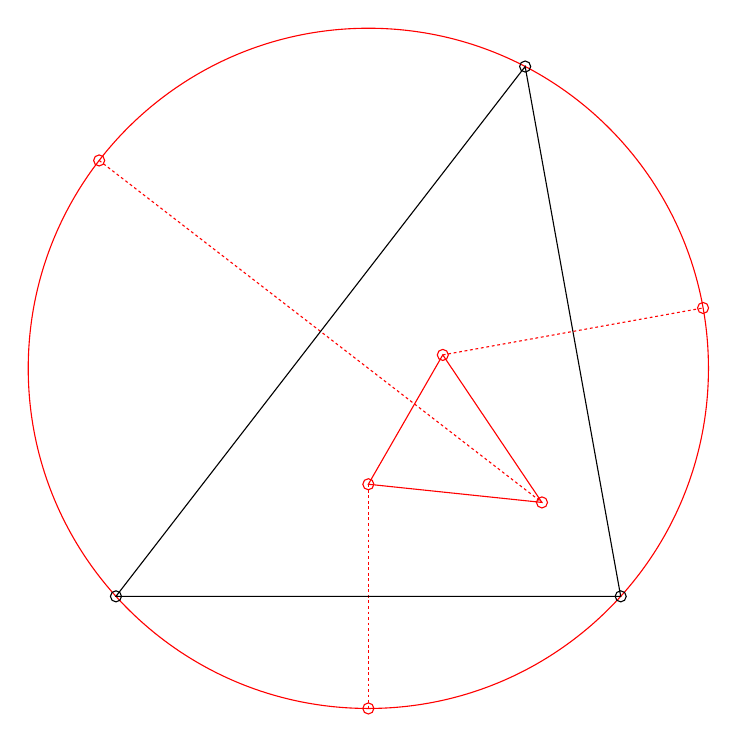
\begin{tikzpicture}[x=1pt,y=1pt]
\draw[red] (142.05,-135.11) circle (122.90);
\draw[red] (142.05,-176.99) -- (204.78,-183.56) -- (168.95,-130.26) -- cycle;
\draw[red, dash pattern=on 1pt] (142.05,-176.99) -- (142.05,-258.01);
\draw[red, dash pattern=on 1pt] (44.78,-59.99) -- (204.79,-183.56);
\draw (50.85,-217.50) circle (2.00);
\draw (233.24,-217.50) circle (2.00);
\draw (198.71,-26.05) circle (2.00);
\draw[red] (44.78,-59.99) circle (2.00);
\draw[red] (263.00,-113.29) circle (2.00);
\draw[red] (142.05,-258.01) circle (2.00);
\draw[red] (168.96,-130.26) circle (2.00);
\draw[red] (142.05,-176.99) circle (2.00);
\draw[red] (204.79,-183.56) circle (2.00);
\draw (50.85,-217.50) -- (233.24,-217.50) -- (198.71,-26.05) -- cycle;
\draw[red, dash pattern=on 1pt] (168.95,-130.26) -- (263.00,-113.29);
\end{tikzpicture}
\end{document}
